% Options for packages loaded elsewhere
\PassOptionsToPackage{unicode}{hyperref}
\PassOptionsToPackage{hyphens}{url}
\PassOptionsToPackage{dvipsnames,svgnames,x11names}{xcolor}
%
\documentclass[
]{article}

\usepackage{amsmath,amssymb}
\usepackage{iftex}
\ifPDFTeX
  \usepackage[T1]{fontenc}
  \usepackage[utf8]{inputenc}
  \usepackage{textcomp} % provide euro and other symbols
\else % if luatex or xetex
  \usepackage{unicode-math}
  \defaultfontfeatures{Scale=MatchLowercase}
  \defaultfontfeatures[\rmfamily]{Ligatures=TeX,Scale=1}
\fi
\usepackage{lmodern}
\ifPDFTeX\else  
    % xetex/luatex font selection
  \setmainfont[]{DejaVuSans}
  \setmonofont[]{DejaVuSansMono}
\fi
% Use upquote if available, for straight quotes in verbatim environments
\IfFileExists{upquote.sty}{\usepackage{upquote}}{}
\IfFileExists{microtype.sty}{% use microtype if available
  \usepackage[]{microtype}
  \UseMicrotypeSet[protrusion]{basicmath} % disable protrusion for tt fonts
}{}
\makeatletter
\@ifundefined{KOMAClassName}{% if non-KOMA class
  \IfFileExists{parskip.sty}{%
    \usepackage{parskip}
  }{% else
    \setlength{\parindent}{0pt}
    \setlength{\parskip}{6pt plus 2pt minus 1pt}}
}{% if KOMA class
  \KOMAoptions{parskip=half}}
\makeatother
\usepackage{xcolor}
\usepackage[margin=1in]{geometry}
\setlength{\emergencystretch}{3em} % prevent overfull lines
\setcounter{secnumdepth}{5}
% Make \paragraph and \subparagraph free-standing
\ifx\paragraph\undefined\else
  \let\oldparagraph\paragraph
  \renewcommand{\paragraph}[1]{\oldparagraph{#1}\mbox{}}
\fi
\ifx\subparagraph\undefined\else
  \let\oldsubparagraph\subparagraph
  \renewcommand{\subparagraph}[1]{\oldsubparagraph{#1}\mbox{}}
\fi

\usepackage{color}
\usepackage{fancyvrb}
\newcommand{\VerbBar}{|}
\newcommand{\VERB}{\Verb[commandchars=\\\{\}]}
\DefineVerbatimEnvironment{Highlighting}{Verbatim}{commandchars=\\\{\}}
% Add ',fontsize=\small' for more characters per line
\usepackage{framed}
\definecolor{shadecolor}{RGB}{241,243,245}
\newenvironment{Shaded}{\begin{snugshade}}{\end{snugshade}}
\newcommand{\AlertTok}[1]{\textcolor[rgb]{0.68,0.00,0.00}{#1}}
\newcommand{\AnnotationTok}[1]{\textcolor[rgb]{0.37,0.37,0.37}{#1}}
\newcommand{\AttributeTok}[1]{\textcolor[rgb]{0.40,0.45,0.13}{#1}}
\newcommand{\BaseNTok}[1]{\textcolor[rgb]{0.68,0.00,0.00}{#1}}
\newcommand{\BuiltInTok}[1]{\textcolor[rgb]{0.00,0.23,0.31}{#1}}
\newcommand{\CharTok}[1]{\textcolor[rgb]{0.13,0.47,0.30}{#1}}
\newcommand{\CommentTok}[1]{\textcolor[rgb]{0.37,0.37,0.37}{#1}}
\newcommand{\CommentVarTok}[1]{\textcolor[rgb]{0.37,0.37,0.37}{\textit{#1}}}
\newcommand{\ConstantTok}[1]{\textcolor[rgb]{0.56,0.35,0.01}{#1}}
\newcommand{\ControlFlowTok}[1]{\textcolor[rgb]{0.00,0.23,0.31}{#1}}
\newcommand{\DataTypeTok}[1]{\textcolor[rgb]{0.68,0.00,0.00}{#1}}
\newcommand{\DecValTok}[1]{\textcolor[rgb]{0.68,0.00,0.00}{#1}}
\newcommand{\DocumentationTok}[1]{\textcolor[rgb]{0.37,0.37,0.37}{\textit{#1}}}
\newcommand{\ErrorTok}[1]{\textcolor[rgb]{0.68,0.00,0.00}{#1}}
\newcommand{\ExtensionTok}[1]{\textcolor[rgb]{0.00,0.23,0.31}{#1}}
\newcommand{\FloatTok}[1]{\textcolor[rgb]{0.68,0.00,0.00}{#1}}
\newcommand{\FunctionTok}[1]{\textcolor[rgb]{0.28,0.35,0.67}{#1}}
\newcommand{\ImportTok}[1]{\textcolor[rgb]{0.00,0.46,0.62}{#1}}
\newcommand{\InformationTok}[1]{\textcolor[rgb]{0.37,0.37,0.37}{#1}}
\newcommand{\KeywordTok}[1]{\textcolor[rgb]{0.00,0.23,0.31}{#1}}
\newcommand{\NormalTok}[1]{\textcolor[rgb]{0.00,0.23,0.31}{#1}}
\newcommand{\OperatorTok}[1]{\textcolor[rgb]{0.37,0.37,0.37}{#1}}
\newcommand{\OtherTok}[1]{\textcolor[rgb]{0.00,0.23,0.31}{#1}}
\newcommand{\PreprocessorTok}[1]{\textcolor[rgb]{0.68,0.00,0.00}{#1}}
\newcommand{\RegionMarkerTok}[1]{\textcolor[rgb]{0.00,0.23,0.31}{#1}}
\newcommand{\SpecialCharTok}[1]{\textcolor[rgb]{0.37,0.37,0.37}{#1}}
\newcommand{\SpecialStringTok}[1]{\textcolor[rgb]{0.13,0.47,0.30}{#1}}
\newcommand{\StringTok}[1]{\textcolor[rgb]{0.13,0.47,0.30}{#1}}
\newcommand{\VariableTok}[1]{\textcolor[rgb]{0.07,0.07,0.07}{#1}}
\newcommand{\VerbatimStringTok}[1]{\textcolor[rgb]{0.13,0.47,0.30}{#1}}
\newcommand{\WarningTok}[1]{\textcolor[rgb]{0.37,0.37,0.37}{\textit{#1}}}

\providecommand{\tightlist}{%
  \setlength{\itemsep}{0pt}\setlength{\parskip}{0pt}}\usepackage{longtable,booktabs,array}
\usepackage{calc} % for calculating minipage widths
% Correct order of tables after \paragraph or \subparagraph
\usepackage{etoolbox}
\makeatletter
\patchcmd\longtable{\par}{\if@noskipsec\mbox{}\fi\par}{}{}
\makeatother
% Allow footnotes in longtable head/foot
\IfFileExists{footnotehyper.sty}{\usepackage{footnotehyper}}{\usepackage{footnote}}
\makesavenoteenv{longtable}
\usepackage{graphicx}
\makeatletter
\def\maxwidth{\ifdim\Gin@nat@width>\linewidth\linewidth\else\Gin@nat@width\fi}
\def\maxheight{\ifdim\Gin@nat@height>\textheight\textheight\else\Gin@nat@height\fi}
\makeatother
% Scale images if necessary, so that they will not overflow the page
% margins by default, and it is still possible to overwrite the defaults
% using explicit options in \includegraphics[width, height, ...]{}
\setkeys{Gin}{width=\maxwidth,height=\maxheight,keepaspectratio}
% Set default figure placement to htbp
\makeatletter
\def\fps@figure{htbp}
\makeatother

\usepackage{booktabs}
\usepackage{longtable}
\usepackage{array}
\usepackage{multirow}
\usepackage{wrapfig}
\usepackage{float}
\usepackage{colortbl}
\usepackage{pdflscape}
\usepackage{tabu}
\usepackage{threeparttable}
\usepackage{threeparttablex}
\usepackage[normalem]{ulem}
\usepackage{makecell}
\usepackage{xcolor}
\makeatletter
\@ifpackageloaded{caption}{}{\usepackage{caption}}
\AtBeginDocument{%
\ifdefined\contentsname
  \renewcommand*\contentsname{Table of contents}
\else
  \newcommand\contentsname{Table of contents}
\fi
\ifdefined\listfigurename
  \renewcommand*\listfigurename{List of Figures}
\else
  \newcommand\listfigurename{List of Figures}
\fi
\ifdefined\listtablename
  \renewcommand*\listtablename{List of Tables}
\else
  \newcommand\listtablename{List of Tables}
\fi
\ifdefined\figurename
  \renewcommand*\figurename{Figure}
\else
  \newcommand\figurename{Figure}
\fi
\ifdefined\tablename
  \renewcommand*\tablename{Table}
\else
  \newcommand\tablename{Table}
\fi
}
\@ifpackageloaded{float}{}{\usepackage{float}}
\floatstyle{ruled}
\@ifundefined{c@chapter}{\newfloat{codelisting}{h}{lop}}{\newfloat{codelisting}{h}{lop}[chapter]}
\floatname{codelisting}{Listing}
\newcommand*\listoflistings{\listof{codelisting}{List of Listings}}
\makeatother
\makeatletter
\makeatother
\makeatletter
\@ifpackageloaded{caption}{}{\usepackage{caption}}
\@ifpackageloaded{subcaption}{}{\usepackage{subcaption}}
\makeatother
\ifLuaTeX
  \usepackage{selnolig}  % disable illegal ligatures
\fi
\usepackage[]{natbib}
\bibliographystyle{plainnat}
\usepackage{bookmark}

\IfFileExists{xurl.sty}{\usepackage{xurl}}{} % add URL line breaks if available
\urlstyle{same} % disable monospaced font for URLs
\hypersetup{
  pdftitle={Towards a principled statistical workflow for the study of wildlife and environmental contaminants in the presence of method detection and quantification limits},
  colorlinks=true,
  linkcolor={blue},
  filecolor={Maroon},
  citecolor={Blue},
  urlcolor={Blue},
  pdfcreator={LaTeX via pandoc}}

\title{Towards a principled statistical workflow for the study of
wildlife and environmental contaminants in the presence of method
detection and quantification limits}
\author{Allen Bush-Beaupré \and Marc Bélisle}
\date{}

\begin{document}
\maketitle

\textsubscript{Source:
\href{https://abushbeaupre.github.io/quantifying_pesticides/index.qmd.html}{Article
Notebook}}

\subsection{Introduction}\label{introduction}

Human industrial and agricultural intensification has resulted in the
release of an astronomical diversity and quantity of contaminants in the
environment. The impact of these contaminants, such as mercury and
pesticides used in agriculture has been the subject of many discussions
in the scientific and public sphere. In her seminal book, Rachel Carson
BLABLA. Much effort has been invested in quantifying the impact of such
contaminants on various life traits in controlled conditions (eg.
BLABLA). Studies such as these are a critical first step in determining
contaminant concentration thresholds at which we may observe the
detrimental impact of human industrial and agricultural activities.
However, the results of these laboratory and semi-field studies can be
difficult to fully extrapolate to the real-life environment conditions
to which organisms are exposed. Organisms are exposed to a diversity of
contaminants depending on their environmental conditions. Additionally,
we would expect an increased level of contamination in organisms at
higher trophic levels due to bioaccumulation.

As emphasized in a review by Tison et al.~(2024), the mechanisms and
consequences by which pesticides accumulate across trophic levels are
understudied. The initial step in studying such phenomena is a proper
quantification of the chemicals in collected samples. Contamination
concentrations are obtained through a variety of laboratory methods.
These methods, however, have varying degrees of precision especially
when concentrations are low. Thus arises the limit of detection (LOD),
the concentration threshold under which the analytical method can not
accurately determine if the contaminant is present in the sample or not.
Additionally, many analytical methods commonly used have a limit of
quantification (LOQ) such that concentrations between the LOD and LOQ
are known to be present, but the actual concentration is only known to
be within the aforementioned interval. As will be exemplified here, much
effort has been made to deal with these complicated data to generate
meaningful statistics for over 50 years (ie Leese, 1973). Methods have
been proposed, validated and their performance compared by multiple
authors (ie Ganser \& Hewett, 2010; Huynh et al.~2014, 2015; Busschaert
et al.~2011; Gilliom, 1986; She, 1997; Hornung \& Reed, 1990; Antweiler
\& Taylor, 2008; Hewett \& Ganser, 2007; Shoari 2016; Sinha, 2006;
Succop et al.~2004; Vlachonikolis \& Marriott, 1995; ). However,
practitioners in the field of ecology often lack the statistical
training to choose and implement an appropriate method for their
specific use cases. Authors often refer to heuristics proposed by others
through simulation studies without considering the specific conditions
involved in those simulations. We propose here a general data analysis
workflow that may be adapted by practitioners for their data at hand
using the most recent advances in statistical software and methods. Such
workflow will encourage researchers to tailor their statistical models
to the specific characteristics of their collected data and make for
easier contrasts among results obtained across various studies.

The accuracy and relevance of the results obtained from modeling efforts
rely on statistical models based on the data-generating process. Such
endeavor implies profound thinking about the characteristics of the data
collected. An example of this in regression models is the use of
likelihood distributions mathematically sound for the data at hand. The
lognormal distribution is often recommended for concentration data as
BLABLA REFS. In the case of contaminants found in wildlife samples,
however, for a concentration level to be known, the contaminant must be
present in the sample in the first place. Thus arises a need for
quantifying the probability of contamination along with the
concentration level if present. Generalized Linear Model (GLM)
likelihoods that may account for this process are part of the hurdle or
zero-inflated class of models. Such models are used, for example, in
occupancy and distribution models (refs). EXAMPLE REF. An additional
aspect of the data-generating process is the limitations imposed by the
methods for detection and quantification of contaminants (the previously
mentioned LOD and LOQ). A proper modeling of the data-generating process
mentioned here may at first glance appear complex and tedious. The next
sections will focus on elaborating the formulation of a statistical
model incorporating the entirety of these specific data characteristics
with reference to approaches taken by researchers in recent publications
(2020-2024) to deal with contaminant presence (often termed exposure)
and concentrations in the presence of LODs and LOQs.

\subsubsection{Data-generating process: limits of detection and
quantification}\label{data-generating-process-limits-of-detection-and-quantification}

Concentration values under LOD and between LOD and LOQ are considered as
censored observations. Censoring in the context of data analysis refers
to inferring BLABLA. These methods are often used in survival analysis
where, for example, we attempt to estimate the survival time of an
individual in a population, but we don't know exactly when death
happened. Such cases arise when we observe individuals over time but do
not get the opportunity to confirm its time of death due to a variety of
reasons such as it leaving the study site, or the study period did not
last long enough to observe the individual's death. Such data are said
to be right-censored as we do not observe certain values on the
right-side of the distribution of survival times. Although we did not
observe the time of death, we know the individual survived at least
until the last time we recorded it. ACTUAL EXAMPLE.

There are two other cases of data censoring. Left-censoring occurs when
we do not observe values past the left side of a given threshold of a
distribution. This may occur, to return to the previous survival time
example, when we do not know the exact age of an individual within a
population and the start of the study. We do, however, have methods to
approximate its maximal age and thus know that the age of the individual
must be below a specific threshold. Lastly, interval-censoring arises
when, for example, an event occurs (such as death) between two sampling
occasions. We thus know that death occurred between two values of time
but are uncertain as to exactly when.

Multiple statistical methods have been developed and used for such data,
with varying levels of impact on the estimation of parameters (such as
the mean). Shaori \& Dubé (2018) reviewed various frequentist and
Bayesian methods for this statistical challenge. Readers are referred to
the aforementioned review for a detailed overview. We focus here mainly
on common practices still observed in recent years by wildlife and
environmental practitioners and build up the reader's intuition for
understanding such data with the objective to fit regression models
evaluating the impact of certain predictors on contaminant presence and
concentration.

\subsubsection{Ignoring values under LOD and/or
LOQ}\label{ignoring-values-under-lod-andor-loq}

One way to work with data under the LOD and/or LOQ is to make the
assumption that these small values are not biologically relevant for the
context at hand. For example, Albert et al.~(2021) measured levels of
Mercury in Arctic seabirds and quantified concentration levels several
orders of magnitude higher than the LOD. In this case, the authors'
assumptions may be justified as the number of samples with concentration
values below the LOD would be unlikely to severely bias the estimation
of concentration levels. There are many contexts, however, where such
assumptions may be detrimental to the precision of the reported
estimated concentrations. For example, when concentration values are
expected to be low such as BLABLA (refs). Additionally, authors have
previously highlighted the bias induced by such methods (Hashimoto \&
Trussel, 1983). While certain studies can justify the choice of data
modifications using toxicological studies in laboratory settings with
known contamination levels and thus use calculations based on samples
exceeding a certain threshold concentration (eg. Odemer et al.~2023),
this does not take into account the half life of these contaminants
which can be low in certain cases (such as neonicotinoids; refs).
Additionally, ignoring lower concentration levels does not aid in
eventually quantifying the effects of these contaminants on the survival
and health parameters of the studied organisms in the wild. Nonetheless,
ignoring detection and/or quantification limits of contamination levels
in wildlife studies remains a common occurrence in recent publications
(Spadetto et al.~2024a, 2024b; Esther et al.~2022; Rial-Berriel et
al.~2021; Martin-Cruz et al.~2024; Fuentes et al.~2023, 2024a, 2024b,
2024c; Bariod et al.~2024; Tison et al.~2023; Lennon et al.~2020b; Lesch
et al.~2024; Badry et al.~2021; Elliot et al.~2024; Drummond et
al.~2024).

\subsubsection{Data substitution or
imputation}\label{data-substitution-or-imputation}

Some practitioners recognize the need to incorporate the information
contained by the samples with concentrations below the LOD or LOQ and
use a variety of methods to substitute values for these points. In
recent years, researchers have substituted observations below either
limit to the median between zero and the limit (Bishops et al.~2022;
Elliot et al.~2022; Perkins et al.~2021), ignored data under the LOD and
set values between LOD and LOQ to LOD (Rondeau et al.~2022) and fixed
values below LOD to LOD (Lennon et al.~2020, Ito et al.~2020). Other
practitioners have used various data imputation methods such as
generating random values between zero and the LOD and between the LOD
and LOQ (Martin-Cruz et al.~2024b). Bias produced by similar practices
have been highlighted in previous publications (Hashimoto \& Trussel,
1983). Another imputation method used is the β-substitution method
(Ganser and Hewett, 2010), used, for example, by Eng et al.~(2020).

\subsubsection{MLE}\label{mle}

Shoari 2016 quantify uncertainty with bootstrap

There exists, however an alternative method to work with censored data
in the Bayesian paradigm. Bayesian models treat uncertainty in a
different manner than Frequentist ones and offer probabilistic
interpretations of parameter values. In a Bayesian paradigm, censored
observations are simply integrated over from the entire data
distribution. This allows the uncertainty of the unobserved values to be
propagated across the entire model and reflected in the width of
confidence intervals generated. When comparing the β-substitution method
to Bayesian left-censoring AUTHORS found the two methods to perform
similarly at low levels of censoring. However, as the number of censored
observations increased, Bayesian left-censoring had a higher predictive
performance. Thus, Bayesian left-censoring allows to model censored data
in a greater variety of cases. Researchers can thus use this method
rather than not model concentrations at all when the level of censored
observations is high such as in the case with METABOLITE in Eng et
al.~(2020). The method has been used in recent publications such as
Kerric et al.~(2022), MORE.

\subsubsection{Data-generating process: Contaminant
presence}\label{data-generating-process-contaminant-presence}

A measure that is often of interest is the probability of exposure that
an environment or organism is subjected to. For example, researchers
often discuss and analyse how the number of pesticides that an
individual is exposed to affects certain life traits. Anderson et
al.~(2023) dichotomized samples above and below the LOQ as a measure of
exposure probability. Due to a lower LOQ for Imidacloprid than the other
pesticides tested, their method of interpretation leads to claiming that
individuals had a higher exposure to Imidacloprid. When analysing a
30-year dataset of rodenticide contamination in raptors, Elliot et
al.~(2022) dealt with detection limits that ranged across several orders
of magnitude by considering only the highest limit and thus quantifying
``exposure'' probability in relation to this value. However, discussing
exposure in the aforementioned manner is erroneous; these measures
relate to inherent imprecisions in the analytical method rather than the
actual data-generating process. Nevertheless, such terminology is
pervasive in recent literature (Rondeau et al.~2022; Fuentes et
al.~2024a, 2024c; Rial-Berriel et al.~2021; Badry et al.~2021; Bischoff
et al.~2023; Martinez et al.~2021; Rodriguez-Aguilar et al.~2022; Roy \&
Chen, 2023; Tison et al.~2023).

\subsubsection{Proposed general statistical
framework}\label{proposed-general-statistical-framework}

Thus far, we have highlighted four major characteristics of
contamination concentration data as illustrated through a simulated data
distribution in Figure~\ref{fig-datagen}. First, there are data that
were properly quantified and are thus observed (ie non-censored; purple
part of distribution). These observations describe the right tail of the
distribution unambiguously. Second, we have observations that lie
between the LOD and LOQ (ie interval-censored; gold part of
distribution). Such data are ambiguous concerning their exact values but
contain valuable information; we know what portion of the distribution
within which they reside. Lastly, we have values below the LOD
(left-censored; red part of distribution) which can be further
characterised into zero-values and values between zero and the LOD. From
the proportion of values located at zero, we may derive an exposure
probability and, from all values above zero, we may derive an average
concentration when the contaminant is present. Furthermore, one may be
inclined to calculate a ``overall'' average thus incorporating the
concentration when present and the contamination probability which can
be obtained by multiplying the two metrics. Although it may appear
counter-intuitive at first, we show here that it is possible to obtain
these metrics from data with such characteristics in a variety of
conditions. We emphasise, however, that practitioners evaluate the
adaptability of the proposed method to their specific use-case following
the workflow provided.

\phantomsection\label{cell-fig-datagen}
\begin{figure}[H]

\centering{

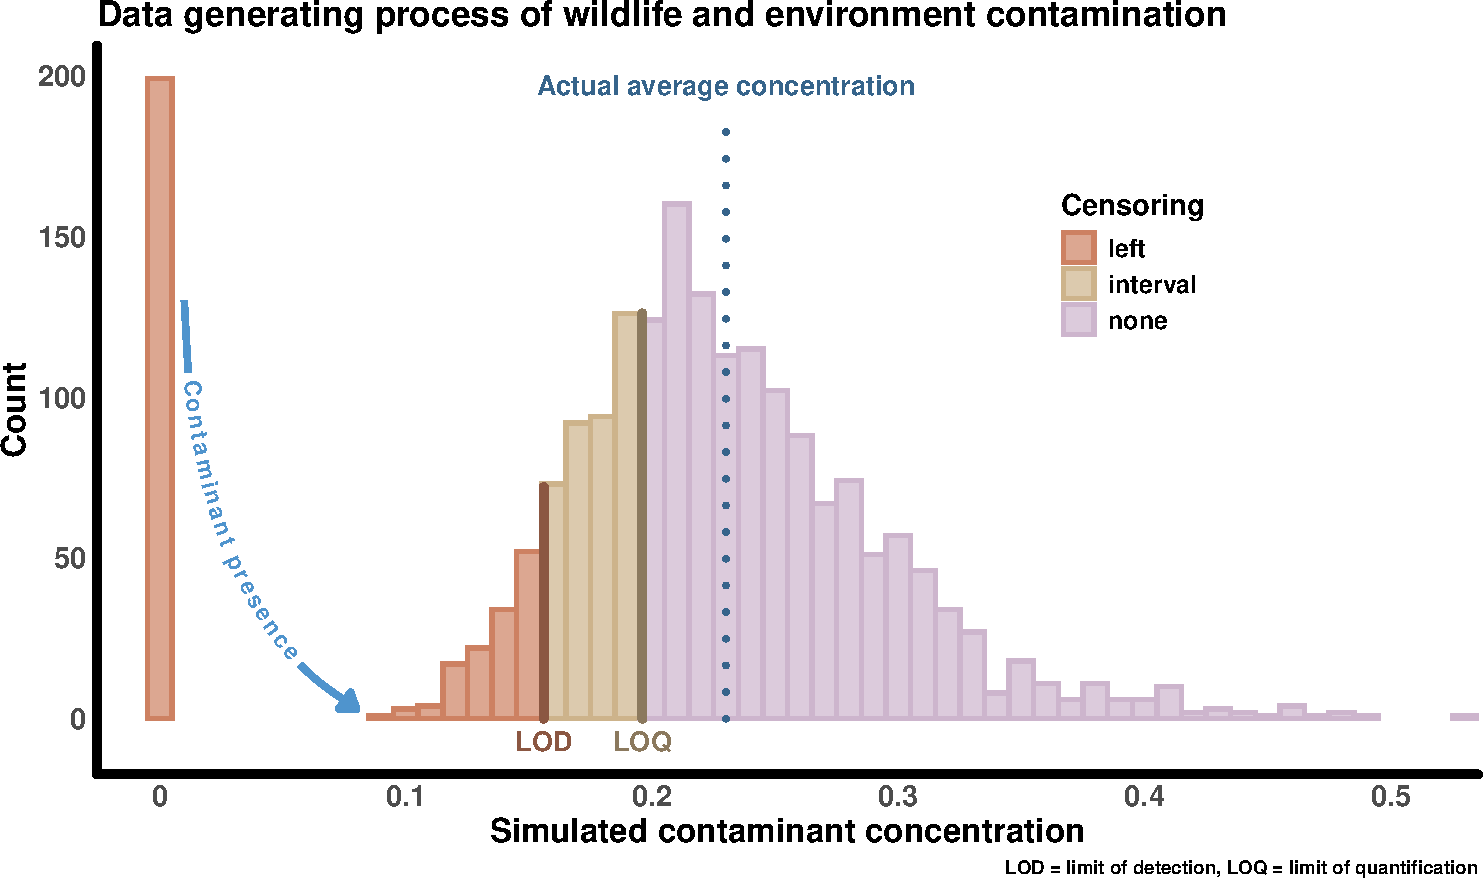
\includegraphics{index_files/figure-pdf/fig-datagen-1.pdf}

}

\caption{\label{fig-datagen}Data generating process of wildlife and
environment sample contamination. The plot shows the distribution of
simulated contaminant concentrations with different censoring regions
highlighted.}

\end{figure}%

\textsubscript{Source:
\href{https://abushbeaupre.github.io/quantifying_pesticides/index.qmd.html}{Article
Notebook}}

Many of the aforementioned studies focus solely on the number of samples
with detected levels of contaminants (refs). Treating the data in such a
manner is problematic as previously emphasized. Others assume a
lognormal distribution and may use any of the mentioned methods to deal
(or not) with the censored data (refs). However, although the lognormal
is theoretically sound for concentration data, it does not allow for
zero-values. Thus, while such models may infer infinitely small
concentrations, an important aspect of the data generating process is
neglected; the probability that the contaminant is present in the sample
in the first place. Model specifications to include the zero-generating
process such as the hurdle lognormal are available and easily
implemented using software such as brms. As will be shown using
simulations and a case study of pesticide contamination in Tree Swallow
boluses, a left- and interval censored hurdle lognormal bayesian
hierarchical generalized linear model can be fit to such data to obtain
contamination probability and concentration with acceptable levels of
precision. As exemplified by the case study, the model can be
complexified to include multiple pesticides along with correlations in
their contamination probability and concentrations, measures of
`cocktail' contaminations.

Setting up a GLMM with censoring is not trivial and requires a deep
understanding of the data-generating process. The next sections will
focus on the formulation of the model and the interpretation of the
results obtained. We will also provide a step-by-step guide to implement
the model using the brms package in R.

\subsection{Data simulation}\label{data-simulation}

To illustrate the proposed statistical workflow, we will simulate a
dataset of contaminant concentrations in wildlife samples. The data will
be generated to mimic the characteristics of real-world data, including
left-censored observations below the limit of detection (LOD) and
interval-censored observations between the LOD and the limit of
quantification (LOQ). The data will be generated from a lognormal
distribution, which is commonly used to model concentration data. The
simulation will also include a binary variable indicating the presence
or absence of the contaminant in each sample. The data distribution
generated can be observed in Figure~\ref{fig-datagen}.

\begin{Shaded}
\begin{Highlighting}[]
\NormalTok{n }\OtherTok{\textless{}{-}} \DecValTok{2000}       \CommentTok{\# Number of samples}
\NormalTok{LOD }\OtherTok{\textless{}{-}} \FloatTok{0.15}     \CommentTok{\# Limit of detection}
\NormalTok{LOQ }\OtherTok{\textless{}{-}} \FloatTok{0.19}     \CommentTok{\# Limit of quantification}
\NormalTok{p\_zeros }\OtherTok{\textless{}{-}} \FloatTok{0.1}  \CommentTok{\# Proportion of zero values}
\CommentTok{\# Generate simulated data}
\NormalTok{censored\_data }\OtherTok{\textless{}{-}} \FunctionTok{tibble}\NormalTok{(}
  \CommentTok{\# Generate lognormal concentrations}
  \AttributeTok{conc =} \FunctionTok{round}\NormalTok{(}\FunctionTok{rlnorm}\NormalTok{(n, }\SpecialCharTok{{-}}\FloatTok{1.5}\NormalTok{, }\FloatTok{0.25}\NormalTok{),}\DecValTok{2}\NormalTok{),  }
  \CommentTok{\# Presence probability of 0.9}
  \AttributeTok{zeros =} \FunctionTok{rbinom}\NormalTok{(n, }\AttributeTok{prob =}\NormalTok{ (}\DecValTok{1} \SpecialCharTok{{-}}\NormalTok{ p\_zeros), }\AttributeTok{size =} \DecValTok{1}\NormalTok{),  }
  \CommentTok{\# Final concentrations (including zeros)}
  \AttributeTok{Y =}\NormalTok{ conc }\SpecialCharTok{*}\NormalTok{ zeros)                        }
\end{Highlighting}
\end{Shaded}

\textsubscript{Source:
\href{https://abushbeaupre.github.io/quantifying_pesticides/index.qmd.html}{Article
Notebook}}

To analyse censored data, \{brms\} requires some pre-processing to
recognize the censored observations. Values below LOD (left-censored)
must be set to LOD while values between LOD and LOQ (interval-censored)
must be set to the lower bound of the interval (LOD). Interval-censoring
also requires additional column must be created to specify the upper
bound of the interval censoring (LOQ) while data that are not censored
are left as is. Finally, a column specifying the type of censoring
(left, interval, none) must be created. The code below performs these
operations on the simulated data.

\begin{Shaded}
\begin{Highlighting}[]
\NormalTok{censored\_data }\SpecialCharTok{|\textgreater{}}
  \FunctionTok{mutate}\NormalTok{(}
    \CommentTok{\# format data}
    \AttributeTok{y\_cen =} \FunctionTok{case\_when}\NormalTok{(}
    \CommentTok{\# Set values below LOD to LOD}
\NormalTok{      Y }\SpecialCharTok{\textless{}}\NormalTok{ LOD }\SpecialCharTok{\textasciitilde{}}\NormalTok{ LOD,  }
    \CommentTok{\# Set values between LOD and LOQ to LOD}
\NormalTok{      Y }\SpecialCharTok{\textgreater{}=}\NormalTok{ LOD }\SpecialCharTok{\&}\NormalTok{ Y }\SpecialCharTok{\textless{}}\NormalTok{ LOQ }\SpecialCharTok{\textasciitilde{}}\NormalTok{ LOD,  }
    \CommentTok{\# Leave other values as is}
      \ConstantTok{TRUE} \SpecialCharTok{\textasciitilde{}}\NormalTok{ Y),  }
    \CommentTok{\# Create column for upper bound of interval censoring}
    \AttributeTok{upper\_int\_cens =} \FunctionTok{ifelse}\NormalTok{(Y }\SpecialCharTok{\textgreater{}=}\NormalTok{ LOD }\SpecialCharTok{\&}\NormalTok{ Y }\SpecialCharTok{\textless{}}\NormalTok{ LOQ, LOQ, Y), }
    \CommentTok{\# Create column for censoring type}
    \AttributeTok{censoring =} \FunctionTok{case\_when}\NormalTok{(}
    \CommentTok{\# Left{-}censored}
\NormalTok{      Y }\SpecialCharTok{\textless{}}\NormalTok{ LOD }\SpecialCharTok{\textasciitilde{}} \StringTok{"left"}\NormalTok{,  }
    \CommentTok{\# Interval{-}censored}
\NormalTok{      Y }\SpecialCharTok{\textgreater{}=}\NormalTok{ LOD }\SpecialCharTok{\&}\NormalTok{ Y }\SpecialCharTok{\textless{}}\NormalTok{ LOQ }\SpecialCharTok{\textasciitilde{}} \StringTok{"interval"}\NormalTok{,  }
    \CommentTok{\# Fully observed}
      \ConstantTok{TRUE} \SpecialCharTok{\textasciitilde{}} \StringTok{"none"}\NormalTok{)  }
\NormalTok{) }\OtherTok{{-}\textgreater{}}\NormalTok{ censored\_data}
\end{Highlighting}
\end{Shaded}

\textsubscript{Source:
\href{https://abushbeaupre.github.io/quantifying_pesticides/index.qmd.html}{Article
Notebook}}

\begin{table}[!h]
\centering
\begin{tabular}{rrrl}
\toprule
Y & y\_cen & upper\_int\_cens & censoring\\
\midrule
0.18 & 0.15 & 0.19 & interval\\
0.15 & 0.15 & 0.19 & interval\\
0.19 & 0.19 & 0.19 & none\\
0.28 & 0.28 & 0.28 & none\\
0.00 & 0.15 & 0.00 & left\\
\addlinespace
0.13 & 0.15 & 0.13 & left\\
\bottomrule
\end{tabular}
\end{table}

\subsection{Model specification with
\{brms\}}\label{model-specification-with-brms}

Next, we specifiy data censoring in the model equation with bf(censored
observations \textbar{} cens(censoring type, upper bound of interval
censoring)). In bf\_intercept below, we specify an intercept-only model
for both the concentration and zero-probability with a hurdle-lognormal
response distribution with identity link for the A parameter, log link
for the B parameter and logit link for the zero-probability.

\begin{Shaded}
\begin{Highlighting}[]
\FunctionTok{library}\NormalTok{(brms)       }\CommentTok{\# Bayesian GLMMs}
\end{Highlighting}
\end{Shaded}

\begin{verbatim}
Loading required package: Rcpp
\end{verbatim}

\begin{verbatim}
Loading 'brms' package (version 2.21.0). Useful instructions
can be found by typing help('brms'). A more detailed introduction
to the package is available through vignette('brms_overview').
\end{verbatim}

\begin{verbatim}

Attaching package: 'brms'
\end{verbatim}

\begin{verbatim}
The following object is masked from 'package:stats':

    ar
\end{verbatim}

\begin{Shaded}
\begin{Highlighting}[]
\FunctionTok{library}\NormalTok{(cmdstanr)   }\CommentTok{\# cmdstanr backend for brms}
\end{Highlighting}
\end{Shaded}

\begin{verbatim}
This is cmdstanr version 0.8.1.9000
\end{verbatim}

\begin{verbatim}
- CmdStanR documentation and vignettes: mc-stan.org/cmdstanr
\end{verbatim}

\begin{verbatim}
- CmdStan path: /home/ubuntu/.cmdstan/cmdstan-2.35.0
\end{verbatim}

\begin{verbatim}
- CmdStan version: 2.35.0
\end{verbatim}

\begin{Shaded}
\begin{Highlighting}[]
\FunctionTok{library}\NormalTok{(tidybayes)  }\CommentTok{\# Extract and visualize priors/posteriors }
\end{Highlighting}
\end{Shaded}

\begin{verbatim}

Attaching package: 'tidybayes'
\end{verbatim}

\begin{verbatim}
The following objects are masked from 'package:brms':

    dstudent_t, pstudent_t, qstudent_t, rstudent_t
\end{verbatim}

\begin{Shaded}
\begin{Highlighting}[]
\NormalTok{bf\_intercept }\OtherTok{\textless{}{-}} \FunctionTok{bf}\NormalTok{(y\_cen }\SpecialCharTok{|} \FunctionTok{cens}\NormalTok{(censoring , upper\_int\_cens) }\SpecialCharTok{\textasciitilde{}} \DecValTok{1}\NormalTok{, }
\NormalTok{                                  hu }\SpecialCharTok{\textasciitilde{}} \DecValTok{1}\NormalTok{, }
                           \AttributeTok{family =} \FunctionTok{hurdle\_lognormal}\NormalTok{(}\AttributeTok{link =} \StringTok{"identity"}\NormalTok{, }\AttributeTok{link\_sigma =} \StringTok{"log"}\NormalTok{, }\AttributeTok{link\_hu =} \StringTok{"logit"}\NormalTok{)}
\NormalTok{)}

\FunctionTok{get\_prior}\NormalTok{(bf\_intercept, }\AttributeTok{data =}\NormalTok{ censored\_data)}
\end{Highlighting}
\end{Shaded}

\begin{verbatim}
               prior     class coef group resp dpar nlpar lb ub  source
\end{verbatim}

student\_t(3, -1.5, 2.5) Intercept default student\_t(3, 0, 2.5) sigma 0
default logistic(0, 1) Intercept hu default

\begin{Shaded}
\begin{Highlighting}[]
\NormalTok{priors\_intercept }\OtherTok{\textless{}{-}} \FunctionTok{c}\NormalTok{(}
  \FunctionTok{prior}\NormalTok{(}\FunctionTok{normal}\NormalTok{(}\DecValTok{0}\NormalTok{,}\DecValTok{2}\NormalTok{), }\AttributeTok{class =} \StringTok{"Intercept"}\NormalTok{, }\AttributeTok{dpar =} \StringTok{"hu"}\NormalTok{),}
  \FunctionTok{prior}\NormalTok{(}\FunctionTok{normal}\NormalTok{(}\DecValTok{0}\NormalTok{, }\FloatTok{2.5}\NormalTok{), }\AttributeTok{class =} \StringTok{"Intercept"}\NormalTok{),}
  \FunctionTok{prior}\NormalTok{(}\FunctionTok{exponential}\NormalTok{(}\FloatTok{0.5}\NormalTok{), }\AttributeTok{class =} \StringTok{"sigma"}\NormalTok{)}
\NormalTok{)}

\NormalTok{prior\_sim\_intercept }\OtherTok{\textless{}{-}} \FunctionTok{brm}\NormalTok{(}\AttributeTok{formula =}\NormalTok{ bf\_intercept,}
                 \AttributeTok{data =}\NormalTok{ censored\_data,}
                 \AttributeTok{prior =}\NormalTok{ priors\_intercept,}
                 \AttributeTok{sample\_prior =} \StringTok{"only"}\NormalTok{,}
                 \AttributeTok{iter =} \DecValTok{2000}\NormalTok{, }\AttributeTok{warmup =} \DecValTok{1000}\NormalTok{, }\AttributeTok{chains =} \DecValTok{4}\NormalTok{, }\AttributeTok{cores =} \DecValTok{4}\NormalTok{,}
                 \AttributeTok{threads =} \FunctionTok{threading}\NormalTok{(}\DecValTok{4}\NormalTok{, }\AttributeTok{grainsize =} \DecValTok{100}\NormalTok{),}
                 \AttributeTok{backend =} \StringTok{"cmdstanr"}\NormalTok{)}
\end{Highlighting}
\end{Shaded}

\begin{verbatim}
Start sampling
\end{verbatim}

Running MCMC with 4 parallel chains, with 4 thread(s) per chain\ldots{}

Chain 1 Iteration: 1 / 2000 {[} 0\%{]} (Warmup) Chain 1 Iteration: 100 /
2000 {[} 5\%{]} (Warmup) Chain 1 Iteration: 200 / 2000 {[} 10\%{]}
(Warmup) Chain 1 Iteration: 300 / 2000 {[} 15\%{]} (Warmup) Chain 1
Iteration: 400 / 2000 {[} 20\%{]} (Warmup) Chain 1 Iteration: 500 / 2000
{[} 25\%{]} (Warmup) Chain 1 Iteration: 600 / 2000 {[} 30\%{]} (Warmup)
Chain 1 Iteration: 700 / 2000 {[} 35\%{]} (Warmup) Chain 1 Iteration:
800 / 2000 {[} 40\%{]} (Warmup) Chain 1 Iteration: 900 / 2000 {[}
45\%{]} (Warmup) Chain 1 Iteration: 1000 / 2000 {[} 50\%{]} (Warmup)
Chain 1 Iteration: 1001 / 2000 {[} 50\%{]} (Sampling) Chain 1 Iteration:
1100 / 2000 {[} 55\%{]} (Sampling) Chain 1 Iteration: 1200 / 2000 {[}
60\%{]} (Sampling) Chain 1 Iteration: 1300 / 2000 {[} 65\%{]} (Sampling)
Chain 1 Iteration: 1400 / 2000 {[} 70\%{]} (Sampling) Chain 1 Iteration:
1500 / 2000 {[} 75\%{]} (Sampling) Chain 1 Iteration: 1600 / 2000 {[}
80\%{]} (Sampling) Chain 1 Iteration: 1700 / 2000 {[} 85\%{]} (Sampling)
Chain 1 Iteration: 1800 / 2000 {[} 90\%{]} (Sampling) Chain 1 Iteration:
1900 / 2000 {[} 95\%{]} (Sampling) Chain 1 Iteration: 2000 / 2000
{[}100\%{]} (Sampling) Chain 2 Iteration: 1 / 2000 {[} 0\%{]} (Warmup)
Chain 2 Iteration: 100 / 2000 {[} 5\%{]} (Warmup) Chain 2 Iteration: 200
/ 2000 {[} 10\%{]} (Warmup) Chain 2 Iteration: 300 / 2000 {[} 15\%{]}
(Warmup) Chain 2 Iteration: 400 / 2000 {[} 20\%{]} (Warmup) Chain 2
Iteration: 500 / 2000 {[} 25\%{]} (Warmup) Chain 2 Iteration: 600 / 2000
{[} 30\%{]} (Warmup) Chain 2 Iteration: 700 / 2000 {[} 35\%{]} (Warmup)
Chain 2 Iteration: 800 / 2000 {[} 40\%{]} (Warmup) Chain 2 Iteration:
900 / 2000 {[} 45\%{]} (Warmup) Chain 2 Iteration: 1000 / 2000 {[}
50\%{]} (Warmup) Chain 2 Iteration: 1001 / 2000 {[} 50\%{]} (Sampling)
Chain 2 Iteration: 1100 / 2000 {[} 55\%{]} (Sampling) Chain 2 Iteration:
1200 / 2000 {[} 60\%{]} (Sampling) Chain 2 Iteration: 1300 / 2000 {[}
65\%{]} (Sampling) Chain 2 Iteration: 1400 / 2000 {[} 70\%{]} (Sampling)
Chain 2 Iteration: 1500 / 2000 {[} 75\%{]} (Sampling) Chain 2 Iteration:
1600 / 2000 {[} 80\%{]} (Sampling) Chain 2 Iteration: 1700 / 2000 {[}
85\%{]} (Sampling) Chain 2 Iteration: 1800 / 2000 {[} 90\%{]} (Sampling)
Chain 2 Iteration: 1900 / 2000 {[} 95\%{]} (Sampling) Chain 2 Iteration:
2000 / 2000 {[}100\%{]} (Sampling) Chain 3 Iteration: 1 / 2000 {[}
0\%{]} (Warmup) Chain 3 Iteration: 100 / 2000 {[} 5\%{]} (Warmup) Chain
3 Iteration: 200 / 2000 {[} 10\%{]} (Warmup) Chain 3 Iteration: 300 /
2000 {[} 15\%{]} (Warmup) Chain 3 Iteration: 400 / 2000 {[} 20\%{]}
(Warmup) Chain 3 Iteration: 500 / 2000 {[} 25\%{]} (Warmup) Chain 3
Iteration: 600 / 2000 {[} 30\%{]} (Warmup) Chain 3 Iteration: 700 / 2000
{[} 35\%{]} (Warmup) Chain 3 Iteration: 800 / 2000 {[} 40\%{]} (Warmup)
Chain 3 Iteration: 900 / 2000 {[} 45\%{]} (Warmup) Chain 3 Iteration:
1000 / 2000 {[} 50\%{]} (Warmup) Chain 3 Iteration: 1001 / 2000 {[}
50\%{]} (Sampling) Chain 3 Iteration: 1100 / 2000 {[} 55\%{]} (Sampling)
Chain 3 Iteration: 1200 / 2000 {[} 60\%{]} (Sampling) Chain 3 Iteration:
1300 / 2000 {[} 65\%{]} (Sampling) Chain 3 Iteration: 1400 / 2000 {[}
70\%{]} (Sampling) Chain 3 Iteration: 1500 / 2000 {[} 75\%{]} (Sampling)
Chain 3 Iteration: 1600 / 2000 {[} 80\%{]} (Sampling) Chain 3 Iteration:
1700 / 2000 {[} 85\%{]} (Sampling) Chain 3 Iteration: 1800 / 2000 {[}
90\%{]} (Sampling) Chain 3 Iteration: 1900 / 2000 {[} 95\%{]} (Sampling)
Chain 3 Iteration: 2000 / 2000 {[}100\%{]} (Sampling) Chain 4 Iteration:
1 / 2000 {[} 0\%{]} (Warmup) Chain 4 Iteration: 100 / 2000 {[} 5\%{]}
(Warmup) Chain 4 Iteration: 200 / 2000 {[} 10\%{]} (Warmup) Chain 4
Iteration: 300 / 2000 {[} 15\%{]} (Warmup) Chain 4 Iteration: 400 / 2000
{[} 20\%{]} (Warmup) Chain 4 Iteration: 500 / 2000 {[} 25\%{]} (Warmup)
Chain 4 Iteration: 600 / 2000 {[} 30\%{]} (Warmup) Chain 4 Iteration:
700 / 2000 {[} 35\%{]} (Warmup) Chain 4 Iteration: 800 / 2000 {[}
40\%{]} (Warmup) Chain 4 Iteration: 900 / 2000 {[} 45\%{]} (Warmup)
Chain 4 Iteration: 1000 / 2000 {[} 50\%{]} (Warmup) Chain 4 Iteration:
1001 / 2000 {[} 50\%{]} (Sampling) Chain 4 Iteration: 1100 / 2000 {[}
55\%{]} (Sampling) Chain 4 Iteration: 1200 / 2000 {[} 60\%{]} (Sampling)
Chain 4 Iteration: 1300 / 2000 {[} 65\%{]} (Sampling) Chain 4 Iteration:
1400 / 2000 {[} 70\%{]} (Sampling) Chain 4 Iteration: 1500 / 2000 {[}
75\%{]} (Sampling) Chain 4 Iteration: 1600 / 2000 {[} 80\%{]} (Sampling)
Chain 4 Iteration: 1700 / 2000 {[} 85\%{]} (Sampling) Chain 4 Iteration:
1800 / 2000 {[} 90\%{]} (Sampling) Chain 4 Iteration: 1900 / 2000 {[}
95\%{]} (Sampling) Chain 4 Iteration: 2000 / 2000 {[}100\%{]} (Sampling)
Chain 1 finished in 0.0 seconds. Chain 2 finished in 0.0 seconds. Chain
3 finished in 0.0 seconds. Chain 4 finished in 0.0 seconds.

All 4 chains finished successfully. Mean chain execution time: 0.0
seconds. Total execution time: 0.4 seconds.

\begin{Shaded}
\begin{Highlighting}[]
\FunctionTok{epred\_rvars}\NormalTok{(prior\_sim\_intercept, }
            \AttributeTok{dpar =} \ConstantTok{TRUE}\NormalTok{, }
            \AttributeTok{newdata =} \FunctionTok{tibble}\NormalTok{(}\AttributeTok{.rows =} \DecValTok{1}\NormalTok{))}
\end{Highlighting}
\end{Shaded}

\section{A tibble: 1 x 4}\label{a-tibble-1-x-4}

\begin{verbatim}
          .epred            mu           hu      sigma
      <rvar[1d]>    <rvar[1d]>   <rvar[1d]> <rvar[1d]>
\end{verbatim}

1 1.9e+35 ± 1.2e+37 -0.015 ± 2.5 0.51 ± 0.31 2 ± 1.9

\begin{Shaded}
\begin{Highlighting}[]
\NormalTok{mod\_intercept }\OtherTok{\textless{}{-}} \FunctionTok{brm}\NormalTok{(}\AttributeTok{formula =}\NormalTok{ bf\_intercept,}
                 \AttributeTok{data =}\NormalTok{ censored\_data,}
                 \AttributeTok{prior =}\NormalTok{ priors\_intercept,}
                 \AttributeTok{sample\_prior =} \StringTok{"yes"}\NormalTok{,}
                 \AttributeTok{iter =} \DecValTok{2000}\NormalTok{, }\AttributeTok{warmup =} \DecValTok{1000}\NormalTok{, }\AttributeTok{chains =} \DecValTok{4}\NormalTok{, }\AttributeTok{cores =} \DecValTok{4}\NormalTok{,}
                 \AttributeTok{threads =} \FunctionTok{threading}\NormalTok{(}\DecValTok{4}\NormalTok{, }\AttributeTok{grainsize =} \DecValTok{100}\NormalTok{),}
                 \AttributeTok{backend =} \StringTok{"cmdstanr"}\NormalTok{)}
\end{Highlighting}
\end{Shaded}

\begin{verbatim}
Start sampling
\end{verbatim}

Running MCMC with 4 parallel chains, with 4 thread(s) per chain\ldots{}

Chain 1 Iteration: 1 / 2000 {[} 0\%{]} (Warmup) Chain 2 Iteration: 1 /
2000 {[} 0\%{]} (Warmup) Chain 3 Iteration: 1 / 2000 {[} 0\%{]} (Warmup)
Chain 4 Iteration: 1 / 2000 {[} 0\%{]} (Warmup) Chain 1 Iteration: 100 /
2000 {[} 5\%{]} (Warmup) Chain 2 Iteration: 100 / 2000 {[} 5\%{]}
(Warmup) Chain 1 Iteration: 200 / 2000 {[} 10\%{]} (Warmup) Chain 3
Iteration: 100 / 2000 {[} 5\%{]} (Warmup) Chain 1 Iteration: 300 / 2000
{[} 15\%{]} (Warmup) Chain 2 Iteration: 200 / 2000 {[} 10\%{]} (Warmup)
Chain 3 Iteration: 200 / 2000 {[} 10\%{]} (Warmup) Chain 1 Iteration:
400 / 2000 {[} 20\%{]} (Warmup) Chain 2 Iteration: 300 / 2000 {[}
15\%{]} (Warmup) Chain 1 Iteration: 500 / 2000 {[} 25\%{]} (Warmup)
Chain 2 Iteration: 400 / 2000 {[} 20\%{]} (Warmup) Chain 3 Iteration:
300 / 2000 {[} 15\%{]} (Warmup) Chain 4 Iteration: 100 / 2000 {[} 5\%{]}
(Warmup) Chain 1 Iteration: 600 / 2000 {[} 30\%{]} (Warmup) Chain 2
Iteration: 500 / 2000 {[} 25\%{]} (Warmup) Chain 3 Iteration: 400 / 2000
{[} 20\%{]} (Warmup) Chain 2 Iteration: 600 / 2000 {[} 30\%{]} (Warmup)
Chain 2 Iteration: 700 / 2000 {[} 35\%{]} (Warmup) Chain 3 Iteration:
500 / 2000 {[} 25\%{]} (Warmup) Chain 1 Iteration: 700 / 2000 {[}
35\%{]} (Warmup) Chain 2 Iteration: 800 / 2000 {[} 40\%{]} (Warmup)
Chain 3 Iteration: 600 / 2000 {[} 30\%{]} (Warmup) Chain 4 Iteration:
200 / 2000 {[} 10\%{]} (Warmup) Chain 2 Iteration: 900 / 2000 {[}
45\%{]} (Warmup) Chain 3 Iteration: 700 / 2000 {[} 35\%{]} (Warmup)
Chain 1 Iteration: 800 / 2000 {[} 40\%{]} (Warmup) Chain 2 Iteration:
1000 / 2000 {[} 50\%{]} (Warmup) Chain 2 Iteration: 1001 / 2000 {[}
50\%{]} (Sampling) Chain 3 Iteration: 800 / 2000 {[} 40\%{]} (Warmup)
Chain 4 Iteration: 300 / 2000 {[} 15\%{]} (Warmup) Chain 2 Iteration:
1100 / 2000 {[} 55\%{]} (Sampling) Chain 3 Iteration: 900 / 2000 {[}
45\%{]} (Warmup) Chain 1 Iteration: 900 / 2000 {[} 45\%{]} (Warmup)
Chain 2 Iteration: 1200 / 2000 {[} 60\%{]} (Sampling) Chain 3 Iteration:
1000 / 2000 {[} 50\%{]} (Warmup) Chain 3 Iteration: 1001 / 2000 {[}
50\%{]} (Sampling) Chain 4 Iteration: 400 / 2000 {[} 20\%{]} (Warmup)
Chain 1 Iteration: 1000 / 2000 {[} 50\%{]} (Warmup) Chain 1 Iteration:
1001 / 2000 {[} 50\%{]} (Sampling) Chain 2 Iteration: 1300 / 2000 {[}
65\%{]} (Sampling) Chain 4 Iteration: 500 / 2000 {[} 25\%{]} (Warmup)
Chain 2 Iteration: 1400 / 2000 {[} 70\%{]} (Sampling) Chain 4 Iteration:
600 / 2000 {[} 30\%{]} (Warmup) Chain 2 Iteration: 1500 / 2000 {[}
75\%{]} (Sampling) Chain 3 Iteration: 1100 / 2000 {[} 55\%{]} (Sampling)
Chain 4 Iteration: 700 / 2000 {[} 35\%{]} (Warmup) Chain 1 Iteration:
1100 / 2000 {[} 55\%{]} (Sampling) Chain 2 Iteration: 1600 / 2000 {[}
80\%{]} (Sampling) Chain 4 Iteration: 800 / 2000 {[} 40\%{]} (Warmup)
Chain 4 Iteration: 900 / 2000 {[} 45\%{]} (Warmup) Chain 2 Iteration:
1700 / 2000 {[} 85\%{]} (Sampling) Chain 3 Iteration: 1200 / 2000 {[}
60\%{]} (Sampling) Chain 4 Iteration: 1000 / 2000 {[} 50\%{]} (Warmup)
Chain 4 Iteration: 1001 / 2000 {[} 50\%{]} (Sampling) Chain 1 Iteration:
1200 / 2000 {[} 60\%{]} (Sampling) Chain 2 Iteration: 1800 / 2000 {[}
90\%{]} (Sampling) Chain 2 Iteration: 1900 / 2000 {[} 95\%{]} (Sampling)
Chain 4 Iteration: 1100 / 2000 {[} 55\%{]} (Sampling) Chain 3 Iteration:
1300 / 2000 {[} 65\%{]} (Sampling) Chain 1 Iteration: 1300 / 2000 {[}
65\%{]} (Sampling) Chain 2 Iteration: 2000 / 2000 {[}100\%{]} (Sampling)
Chain 3 Iteration: 1400 / 2000 {[} 70\%{]} (Sampling) Chain 4 Iteration:
1200 / 2000 {[} 60\%{]} (Sampling) Chain 4 Iteration: 1300 / 2000 {[}
65\%{]} (Sampling) Chain 2 finished in 2.2 seconds. Chain 1 Iteration:
1400 / 2000 {[} 70\%{]} (Sampling) Chain 1 Iteration: 1500 / 2000 {[}
75\%{]} (Sampling) Chain 3 Iteration: 1500 / 2000 {[} 75\%{]} (Sampling)
Chain 4 Iteration: 1400 / 2000 {[} 70\%{]} (Sampling) Chain 1 Iteration:
1600 / 2000 {[} 80\%{]} (Sampling) Chain 3 Iteration: 1600 / 2000 {[}
80\%{]} (Sampling) Chain 4 Iteration: 1500 / 2000 {[} 75\%{]} (Sampling)
Chain 1 Iteration: 1700 / 2000 {[} 85\%{]} (Sampling) Chain 3 Iteration:
1700 / 2000 {[} 85\%{]} (Sampling) Chain 4 Iteration: 1600 / 2000 {[}
80\%{]} (Sampling) Chain 1 Iteration: 1800 / 2000 {[} 90\%{]} (Sampling)
Chain 3 Iteration: 1800 / 2000 {[} 90\%{]} (Sampling) Chain 4 Iteration:
1700 / 2000 {[} 85\%{]} (Sampling) Chain 1 Iteration: 1900 / 2000 {[}
95\%{]} (Sampling) Chain 3 Iteration: 1900 / 2000 {[} 95\%{]} (Sampling)
Chain 4 Iteration: 1800 / 2000 {[} 90\%{]} (Sampling) Chain 1 Iteration:
2000 / 2000 {[}100\%{]} (Sampling) Chain 3 Iteration: 2000 / 2000
{[}100\%{]} (Sampling) Chain 4 Iteration: 1900 / 2000 {[} 95\%{]}
(Sampling) Chain 4 Iteration: 2000 / 2000 {[}100\%{]} (Sampling) Chain 1
finished in 2.8 seconds. Chain 3 finished in 2.8 seconds. Chain 4
finished in 2.8 seconds.

All 4 chains finished successfully. Mean chain execution time: 2.7
seconds. Total execution time: 3.0 seconds.

\begin{Shaded}
\begin{Highlighting}[]
\FunctionTok{epred\_rvars}\NormalTok{(mod\_intercept, }
            \AttributeTok{dpar =} \ConstantTok{TRUE}\NormalTok{, }
            \AttributeTok{newdata =} \FunctionTok{tibble}\NormalTok{(}\AttributeTok{.rows =} \DecValTok{1}\NormalTok{))}
\end{Highlighting}
\end{Shaded}

\section{A tibble: 1 x 4}\label{a-tibble-1-x-4-1}

\begin{verbatim}
      .epred             mu              hu          sigma
  <rvar[1d]>     <rvar[1d]>      <rvar[1d]>     <rvar[1d]>
\end{verbatim}

1 0.21 ± 0.0022 -1.5 ± 0.0074 0.085 ± 0.0095 0.25 ± 0.0058

\section*{References}\label{references}
\addcontentsline{toc}{section}{References}

\renewcommand{\bibsection}{}
\bibliography{references.bib}




\end{document}
